
\documentclass[11pt,letterpaper]{article}

\usepackage[utf8]{inputenc}
\usepackage[T1]{fontenc}
\usepackage{lmodern}
\usepackage{amsmath,amssymb,amsfonts,amsthm}
\usepackage{mathtools}
\usepackage{bm}
\usepackage{graphicx}
\usepackage{float}
\usepackage{subcaption}
\usepackage{booktabs}
\usepackage[margin=0.85in]{geometry}
\usepackage{microtype}
\usepackage{enumitem}
\usepackage{titlesec}
\usepackage[hidelinks]{hyperref}

\setlength{\parindent}{0pt}
\setlength{\parskip}{5pt}

\titlespacing*{\section}{0pt}{10pt}{4pt}
\titlespacing*{\subsection}{0pt}{7pt}{3pt}

\newcommand{\R}{\mathbb{R}}
\newcommand{\norm}[1]{\left\lVert #1 \right\rVert}
\newcommand{\grad}{\nabla}
\newcommand{\lap}{\Delta}
\newcommand{\uvec}{\bm{u}}

\title{\vspace{-1.5cm}
    \textbf{Numerical Solution of the 2D Stokes Equations}\\
    \large Staggered Grid Discretization
}
\author{Luciano Henriquez}

\begin{document}

\maketitle
\vspace{-0.6cm}

% --------------------------------------------------
\section{Introduction}
% --------------------------------------------------

We consider the two-dimensional Stokes equations
\begin{equation}
    \begin{aligned}
        \mu \lap \uvec - \grad P &= \bm{b},\\
        \grad \cdot \uvec &= 0,
    \end{aligned}
  \end{equation}
  Where $\uvec$ is the velocity vector of the fluid, defined as $\uvec = [U(x,y),V(x,y)]$, whose components are the $x$ and $y$ components of the velocity, respectively. We also assume $\mu = 1$ and
 we impose periodic boundary conditions for $U,V,P$ on the left and right boundaries, Dirichlet conditions for $U$ in the $y$ direction where $U = 0$ on top and bottom boundaries, and Dirichlet conditions for $V$ in the $y$ direction, where $V = -3.5$ units on our top and bottom boundaries. We discretize the equations on a staggered (MAC) grid and write the discrete unknowns and their boundary conditions as a sparse saddle point system.

% --------------------------------------------------
\section{Numerical Method}
% --------------------------------------------------

We use the method of manufactured solutions to solve the problem. We are given:
\begin{align*}
  U_{an}(x,y) &= \sin (2\pi y)\sin (2\pi x),\\
  V_{an}(x,y) &= -3.5 + \cos (2\pi x)(\cos(2\pi y)-1), \\
  P_{an}(x,y) &= \sin (2\pi y)\cos (2\pi x).
\end{align*}
We can now compute the forcing functions. We get:
\begin{align*}
  f(x,y) &= (-8\pi ^2 +2\pi )\sin (2\pi y)\sin (2\pi x), \\
  g(x,y) &= \cos (2\pi x)[4\pi ^2 -(8\pi ^2 +2\pi )\cos(2\pi y)].
\end{align*}
We can thus let $N_{x}=N_{y}=N$ and $h=1/N$ and construct the MAC grid where $U_{i,j}$ is stored at coordinates $(ih, (h-1/2)h)$, $V_{i,j}$ stored at $((i-1/2)h, jh)$, and $P_{i,j}$ stored at $((i-1/2)h, (j-1/2)h)$. We have pressure located at cell centers, $x$ velocity on left and right faces of pressure cells, and $y$ velocities on top and bottom faces of pressure cells.

We then construct
\begin{align*}
\begin{bmatrix}
  \mu \mathcal{L}_{u} & 0 & -G_{x} \\
  0 & \mu \mathcal{L}_{y} & -G_{y} \\
  D_{x} & D_{y} & 0
\end{bmatrix}
\end{align*}
in matlab, with prescribed velocity values moved to the right hand side of the system at boundaries. Since pressure is not unique, we prescribe the pressure at one grid point $P_{1,1}=0$. We then use backslash to solve.

% --------------------------------------------------
\section{Results and Error Analysis}
% --------------------------------------------------

The following graph is the solution plot of the magnitude of $\uvec$ attained from solving the system in Matlab using backslash:
  \begin{figure}[H]
     \centering
     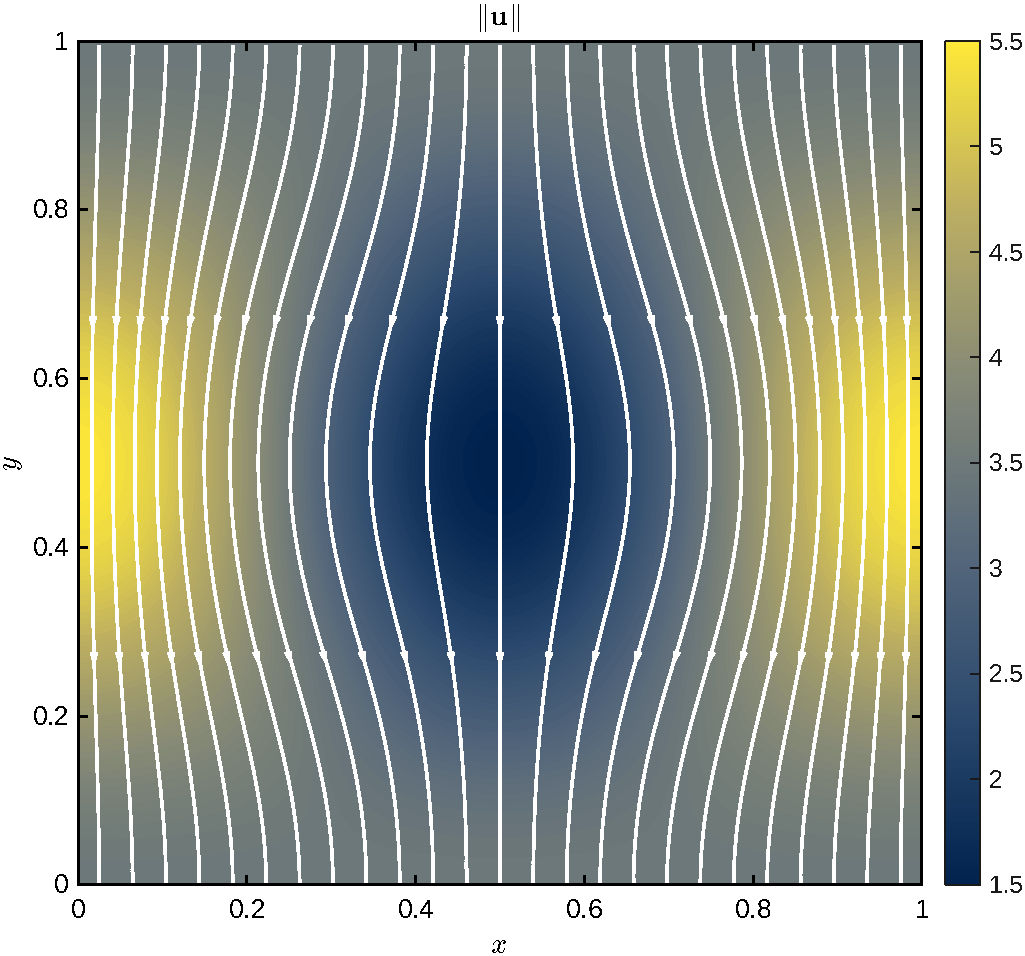
\includegraphics[width=0.6\linewidth]{stokes_velocity.pdf}
     \caption{Solution plot of magnitude of $\uvec$}
     \label{fig:velocity}
   \end{figure}

Figure 1 illustrates the magnitude of $\lVert \uvec \rVert = \sqrt{ U^2+V^2 }$. The streamlines indicate the direction of fluid flow. The flow is downward, consistent with prescribed boundary condition for the vertical velocity, $V=-3.5$. The velocity magnitude is smallest near the center, while reaching a maximum near the x boundaries.

The relative error is defined by
\begin{equation}
    E_U =
    \frac{\norm{U_{\mathrm{num}}-U_{\mathrm{an}}}_2}
         {\norm{U_{\mathrm{an}}}_2}.
\end{equation}

  \begin{figure}[H]
     \centering
     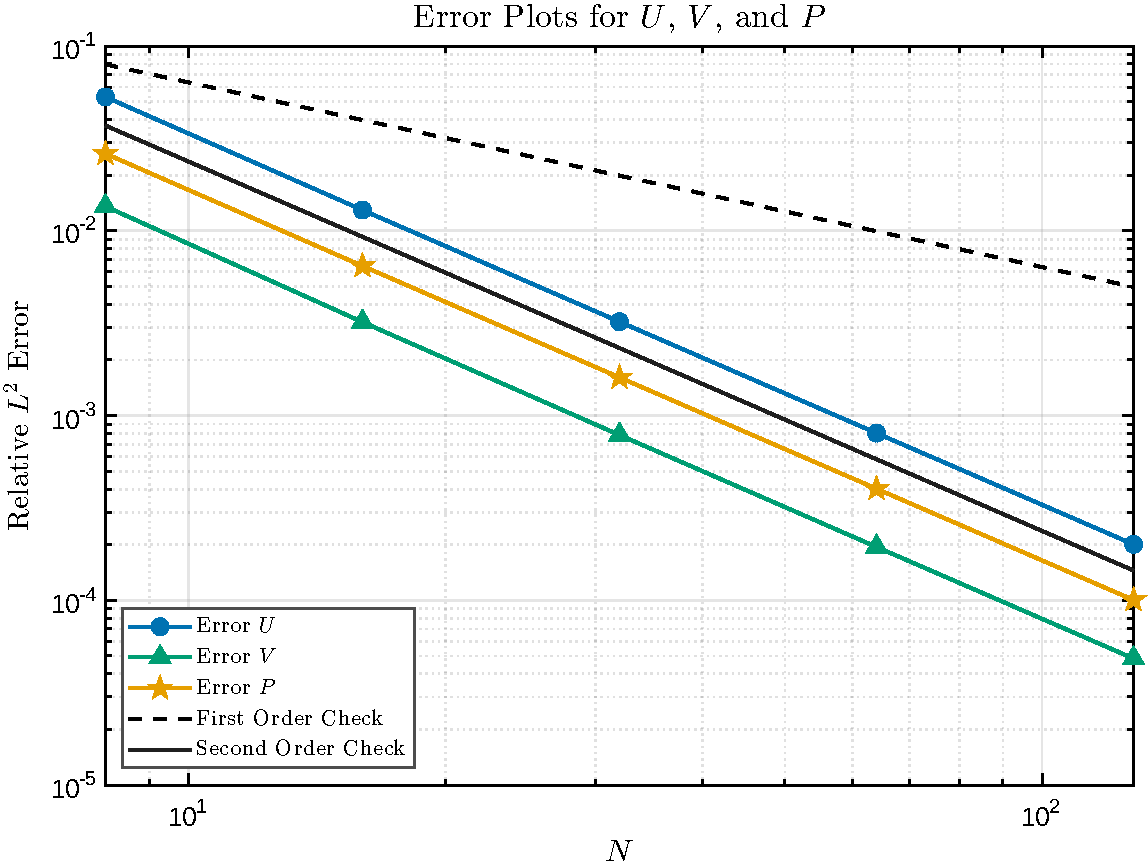
\includegraphics[width=0.6\linewidth]{stokes_errors.pdf}
     \caption{Relative error versus grid resolution.}
     \label{fig:error}
   \end{figure}

Figure 2 graphs the $L^2$ errors for $U,V$, and $P$ as the $N$ grows. All errors decrease with increasing $N$, roughly proportional to $1/N^2$, as can be seen by comparing the slopes of the second order check with the slopes of the errors of $U,V,$ and $P$. This confirms that our MAC discretization is a second order approximation for the manufactured solution.


% --------------------------------------------------
\section{Additional Experiment}
% --------------------------------------------------

We now wish to model flow through some idealized 2d porous microstructure such as circular obstacles. However, using a MAC grid with obstacle masks for instance gives rise to complicated obstacle boundaries. We choose to instead approximate solid boundaries using a method known as Brinkman Penalization to preserve the structure of the existing code, while still simulating flow in porous microstructure. Instead of the original system, we solve:
\begin{align*}
  -\mu \Delta \uvec + \grad p + \alpha (x)\uvec = f\\
  \grad \cdot \uvec = 0
\end{align*}

where
\begin{align*}
  \alpha (x) =
  \begin{cases}
    0 & x\in \Omega _{f}, \\
    \alpha _{s} & x\in \Omega _{s}
  \end{cases}
\end{align*}
where $\alpha _{s}$ is large, $\Omega $ is $[0,1]\times [0,1]$, $\Omega _{f} $ is the region without the obstacle, and $\Omega_{s} $ is the union of regions inside a solid obstacle. This $\alpha $ term suppresses velocity inside solid regions, and so approximates flow in a porous microstructure. Instead of the boundary condition $V=-3.5$, it's better to use a constant vertical body force and periodic boundary conditions in both directions. We thus solve
\begin{align*}
  \mu \Delta \uvec - \grad p - \alpha (x,y) \uvec = -F\\
  \grad \cdot \uvec = 0
\end{align*}

with $\mu  =1$, $ F=(0,-1)$, and $\alpha _{s} =10^5$

Adapting the solution above to the new problem, we get:

  \begin{figure}[H]
     \centering
     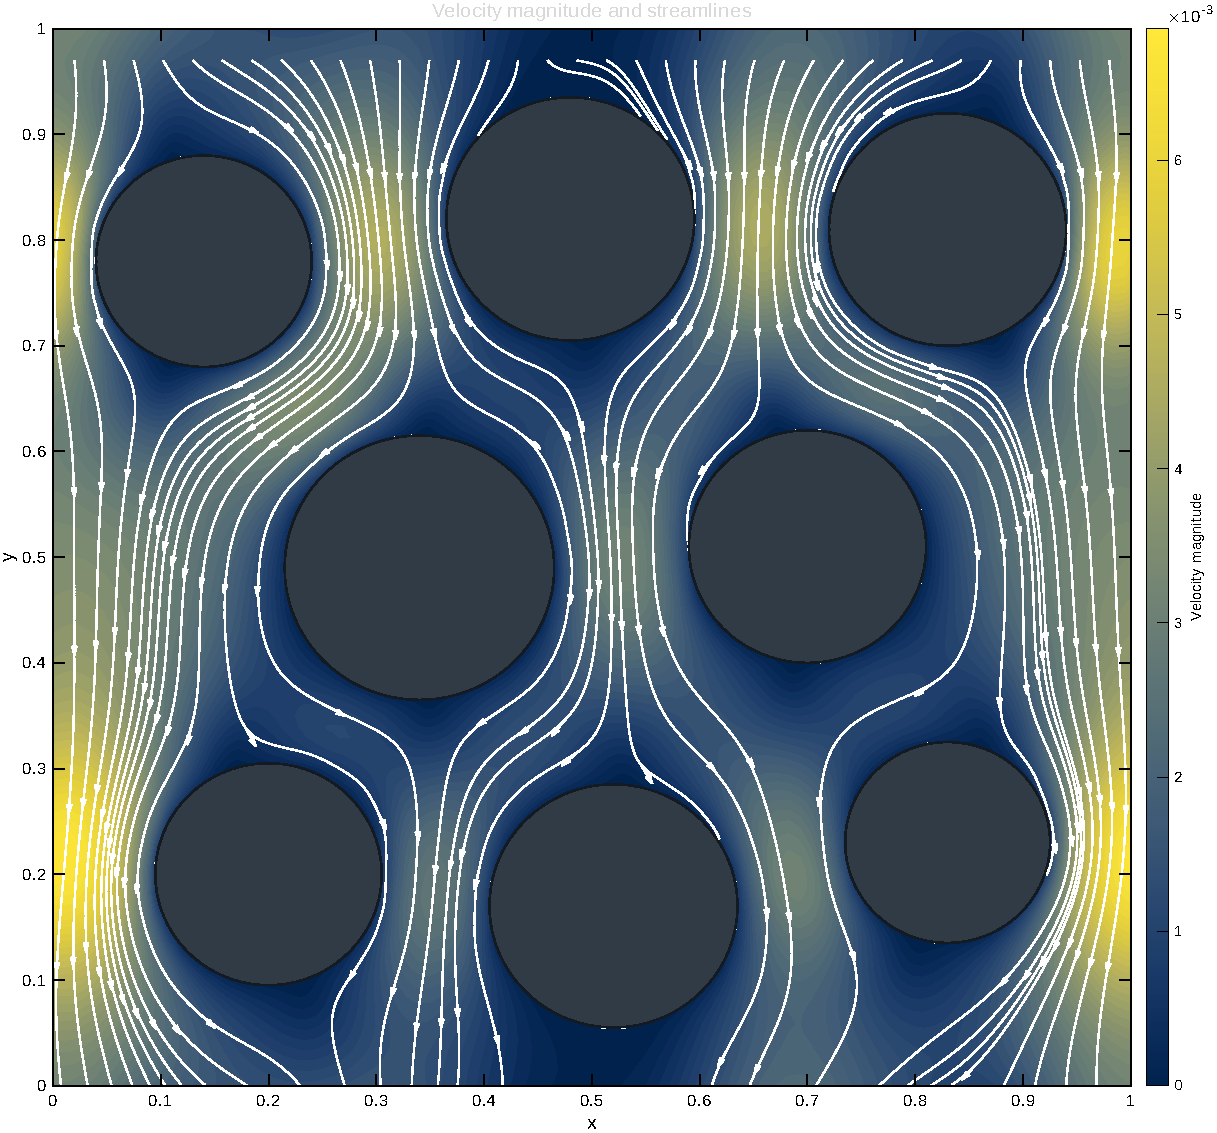
\includegraphics[width=0.6\linewidth]{porous_velocity.pdf}
     \caption{Solution plot of magnitude of $\uvec$ for the porous medium experiment}
     \label{fig:porous_velocity}
   \end{figure}

   Figure 3 showcases the simulation of incompressible fluid flow through a porous microstructure. The contours demonstrate that fluid is redirected around the circular obstacles, with the flow between obstacles having a higher velocity magnitude (due to incompressibility constraint). The velocities are effectively 0 within the obstacles, and is reduced near the obstacles due to the penalization.

% --------------------------------------------------
\section{AI Use Disclosure}
% --------------------------------------------------
AI was used to learn about MAC discretization, as well as to plot all the graphs in the conventions required by the class. In particular, ChatGPT wrote all the matlab code to generate figures 1,2 and 3. ChatGPT was also used to learn about the Brinkman Equations as a good way of approximating flow through a porous microstructure. GLM 5.3 Flash with Opencode harness was used for debugging solver code, directly repairing broken code sections, as well as adding comments and structuring the Matlab code into sections. GLM 5.3 Flash also read the project directory and generated the README.md.

\end{document}
